
\section{Seasonal and Spatial Variation}

\subsection{Springs changing concentration with season, indicating monsoonal precipitation influence}
Time series spring concentration also changing over time Concentration increases then decreases with monsoon.

\begin{figure}[h]
    \centering
    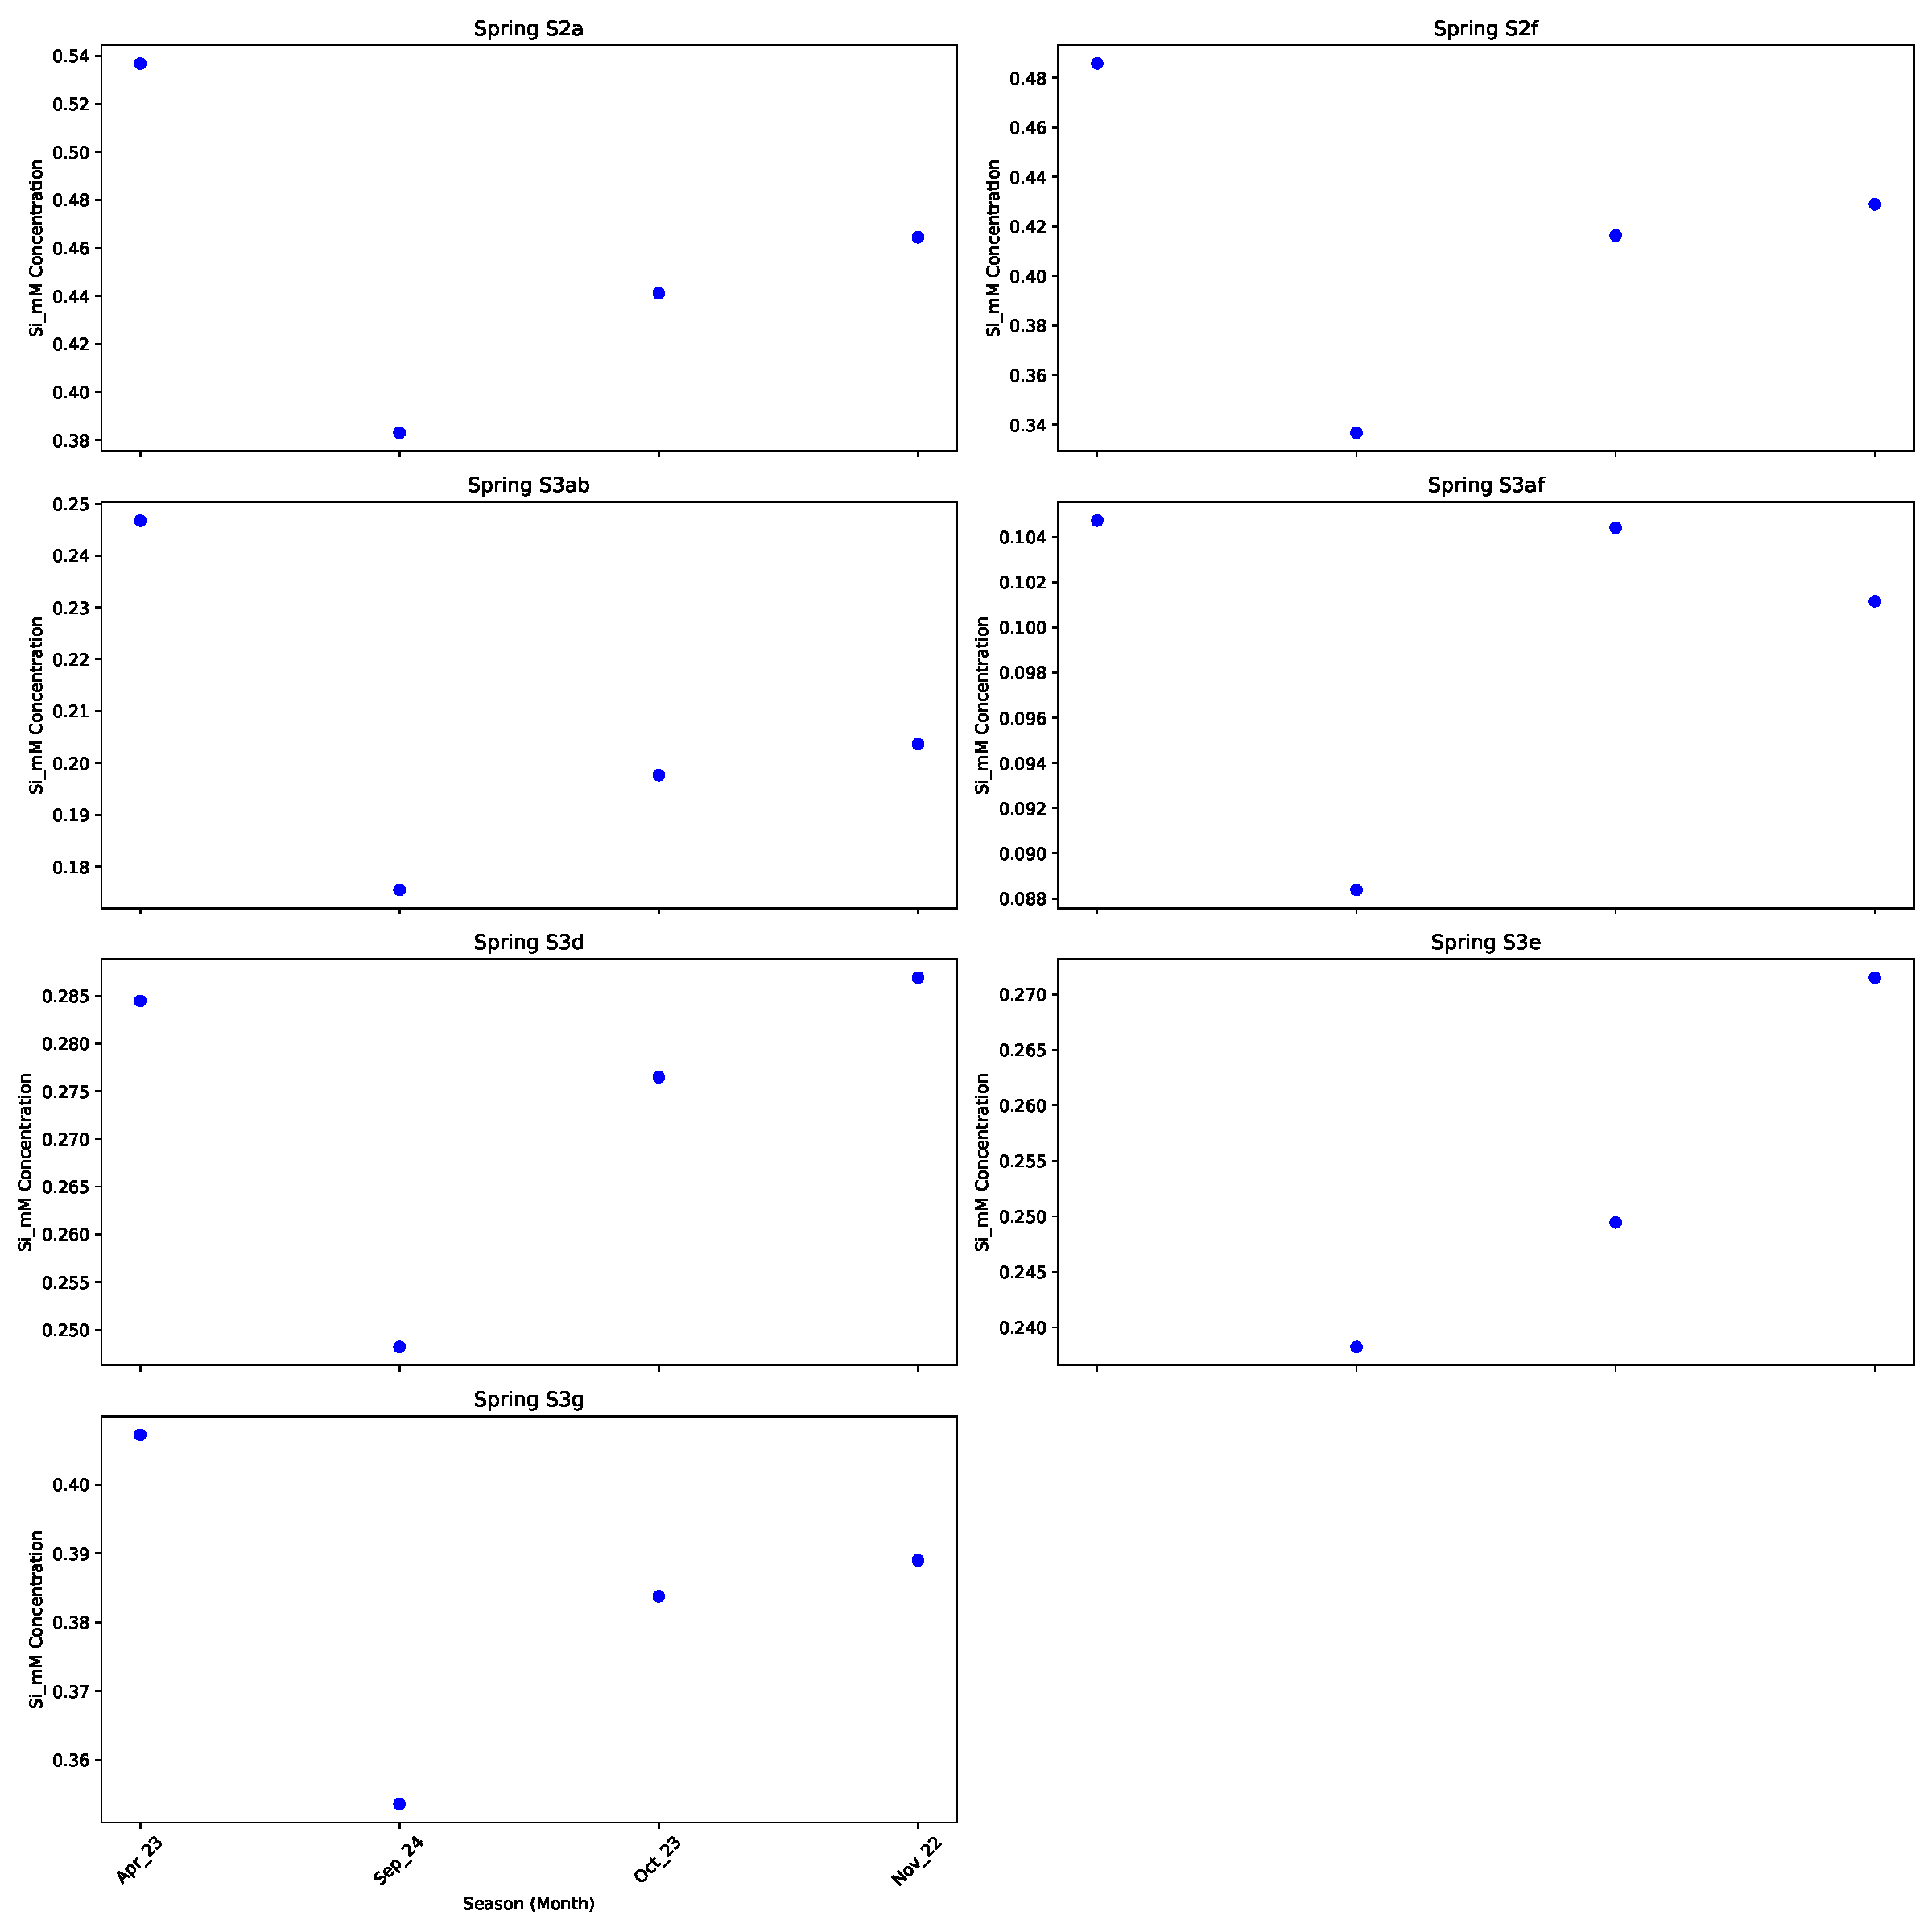
\includegraphics[width=0.6\textwidth]{Si_mM_concentrations_springs.pdf}
    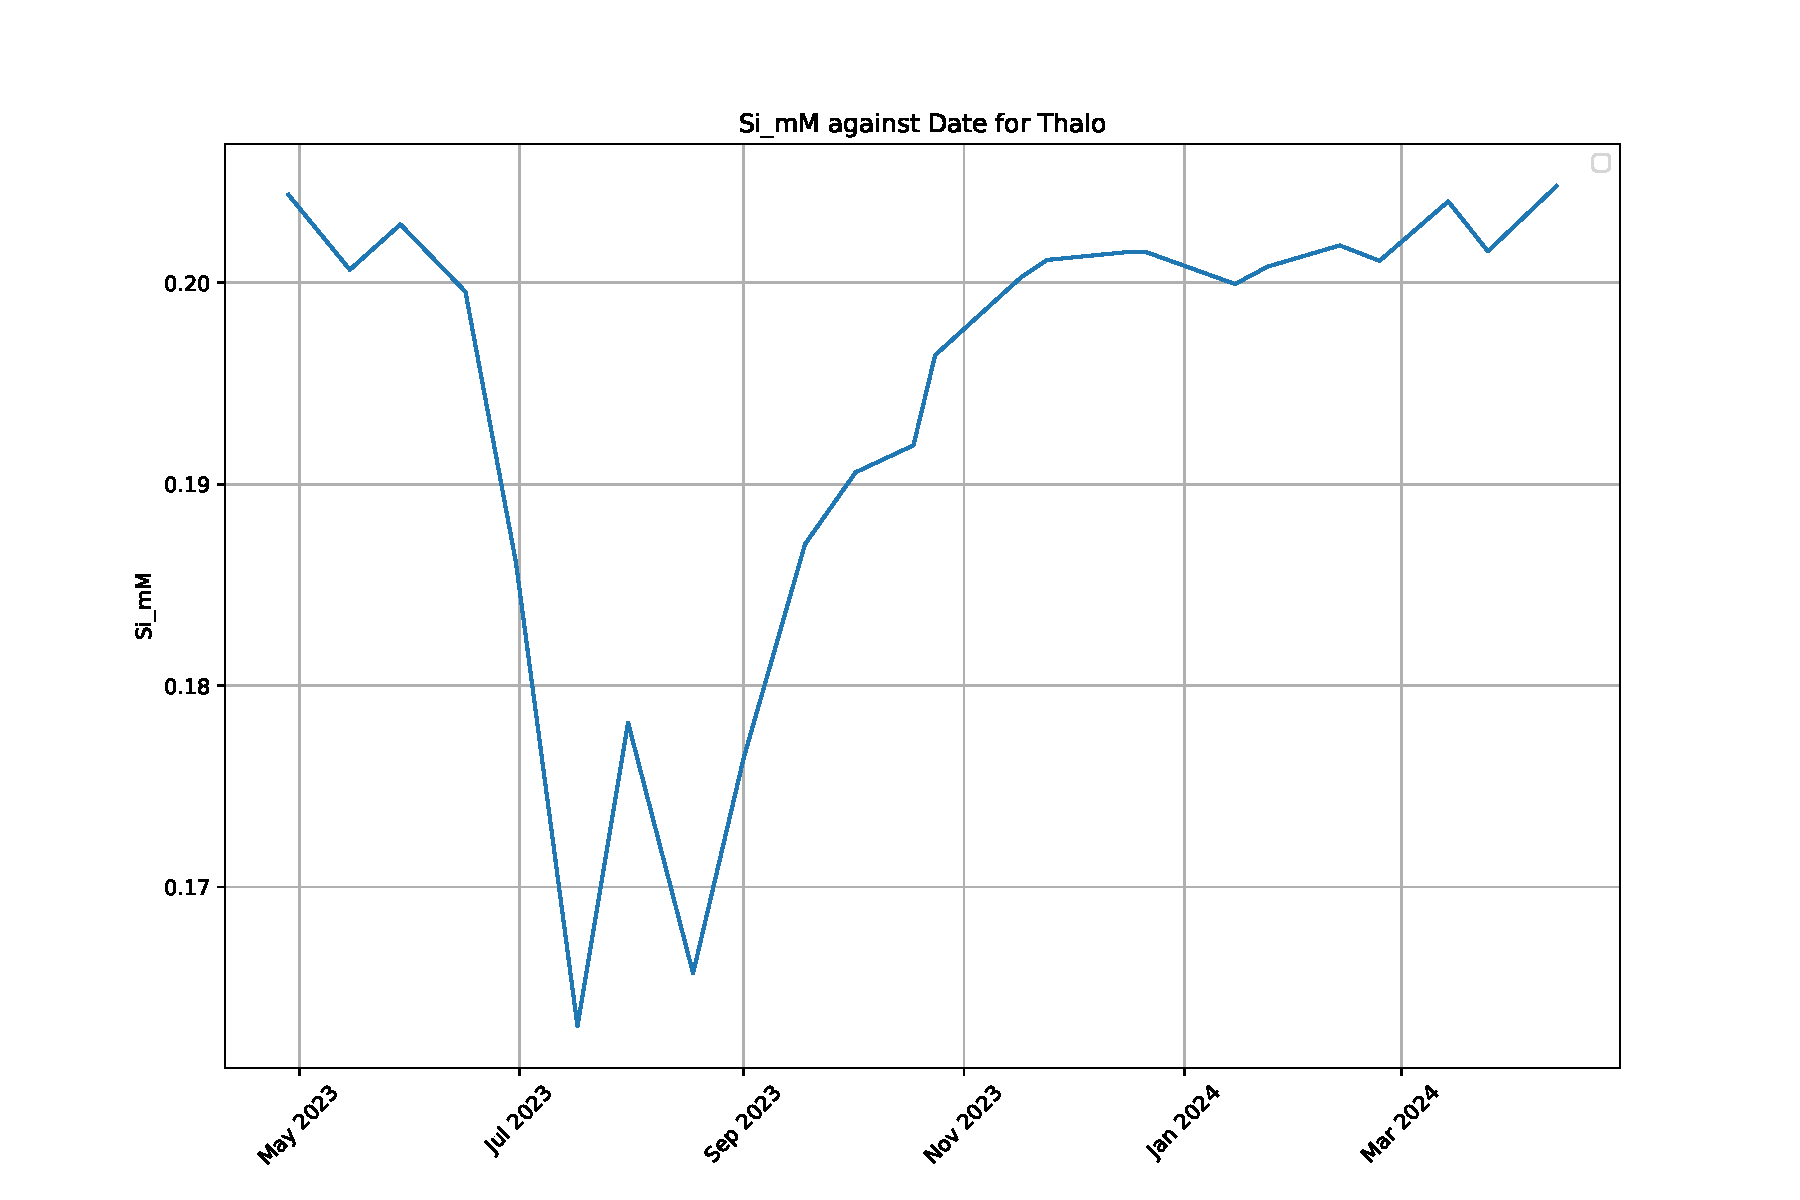
\includegraphics[width=0.8\textwidth]{Si_mM_Thalo_timeseries.pdf}
    \caption{Seasonal changes in spring concentration indicating monsoonal precipitation influence.; Time series of spring concentration changes over time.}
    \label{fig:time_series_changes}
\end{figure}

\FloatBarrier

\begin{figure}[h]
    \centering
    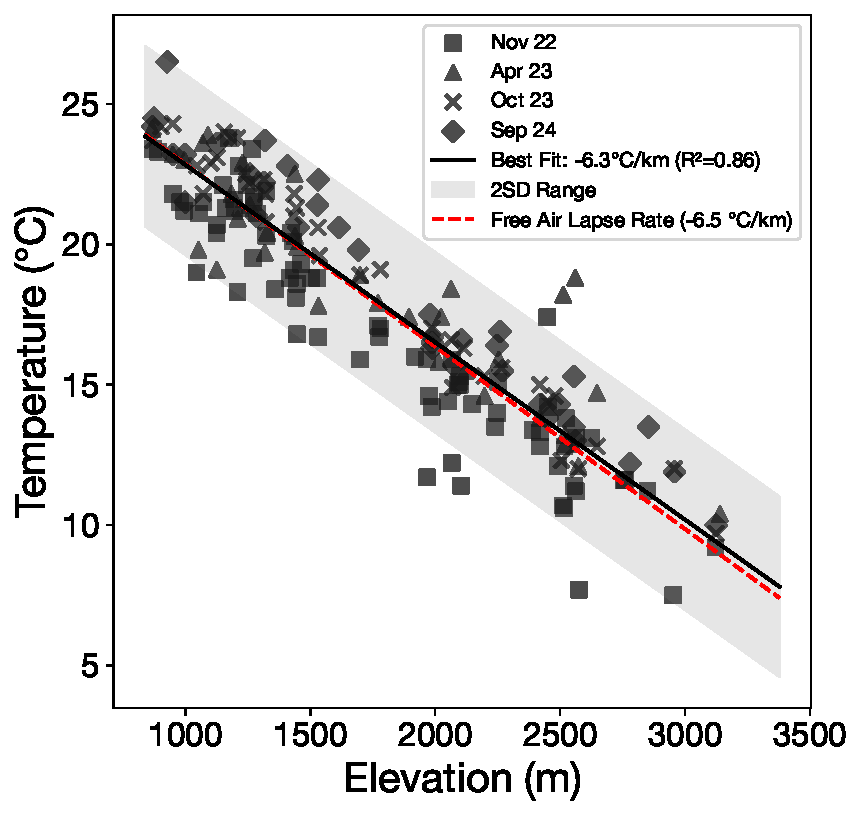
\includegraphics[width=\textwidth]{Temperature_Elevation_Season.pdf}
    \caption{Temperature cahnges}
    \label{fig:seasonal_change2}
\end{figure}

\FloatBarrier



\subsection{Spatial concentration changes between the springs}

\begin{figure}[h]
    \centering
    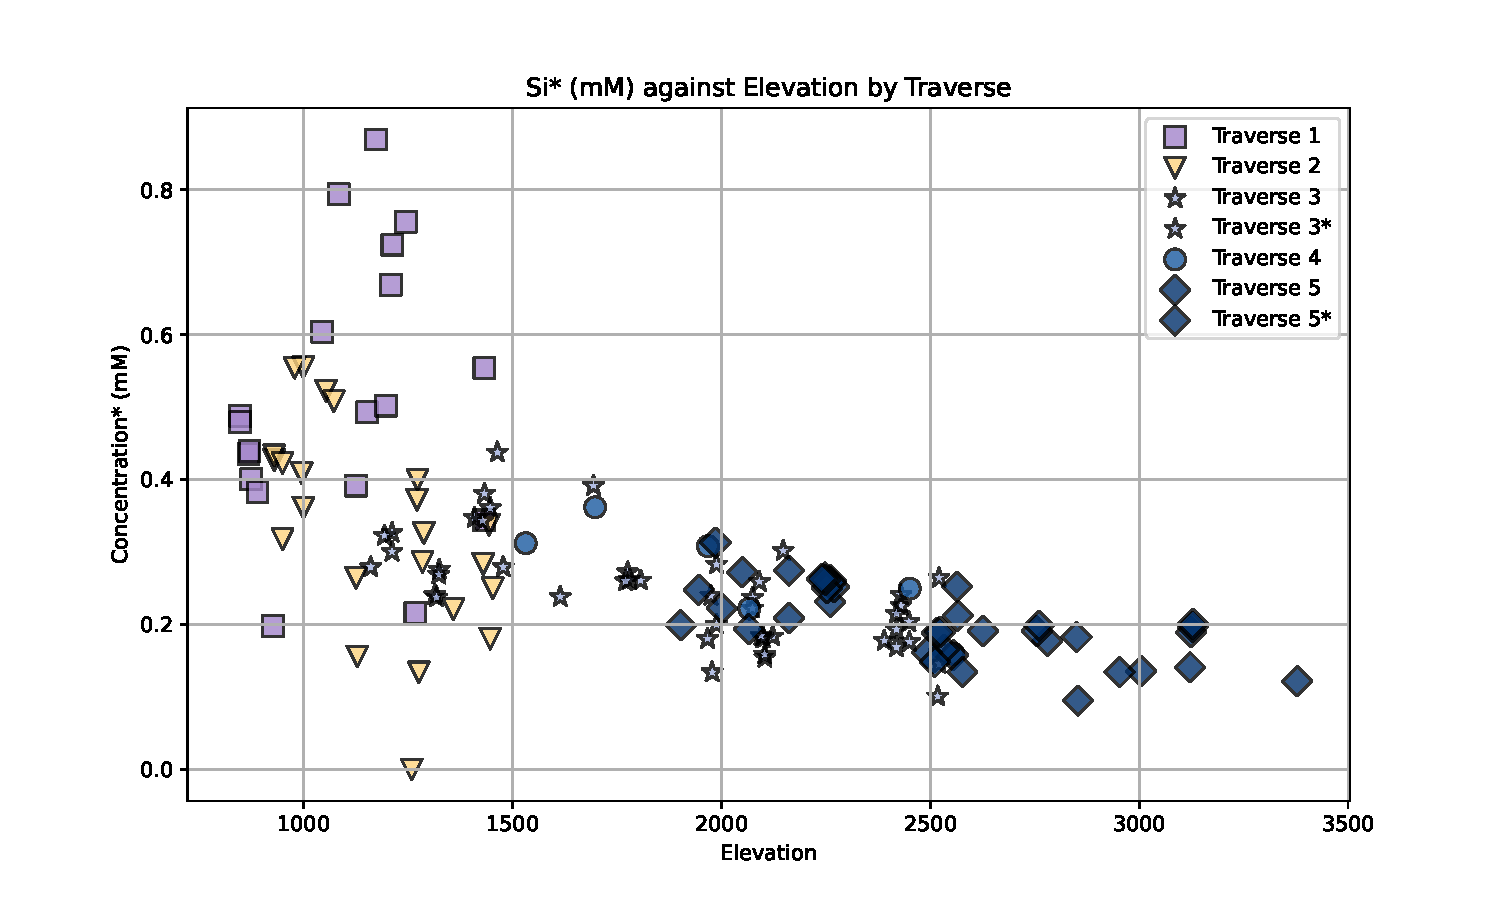
\includegraphics[width=\textwidth]{Si_mM_EC_Elevation.pdf}
    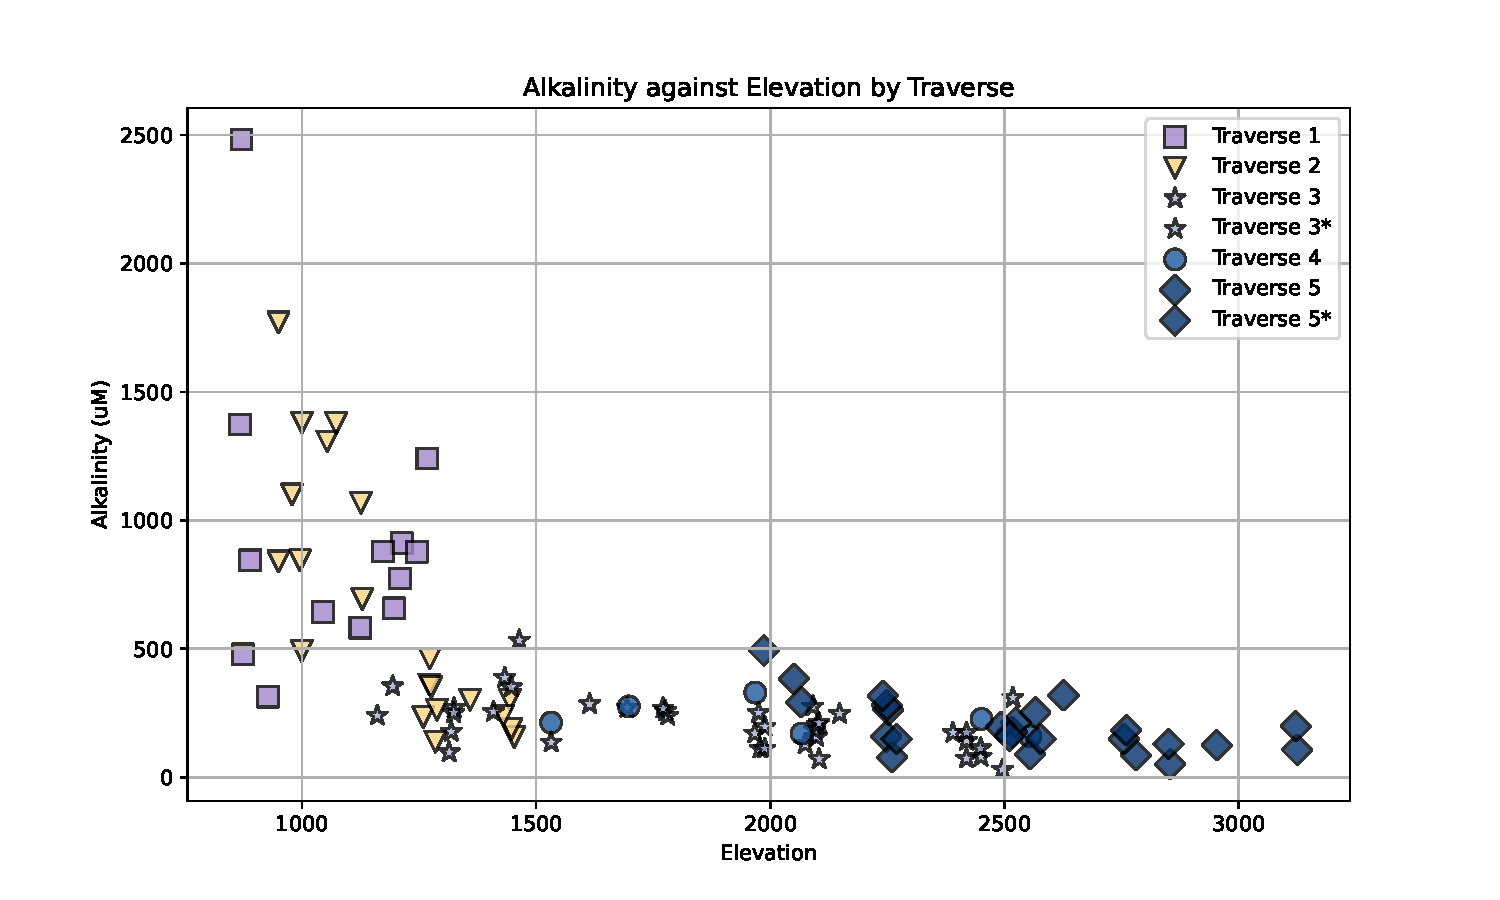
\includegraphics[width=\textwidth]{Alkalinity_Elevation.pdf}
    \caption{How Alkalinity and Si changes with elevation}
    \label{fig:spatial_changes_spring2}
\end{figure}

\FloatBarrier

% \begin{figure}[h]
%     \centering
%     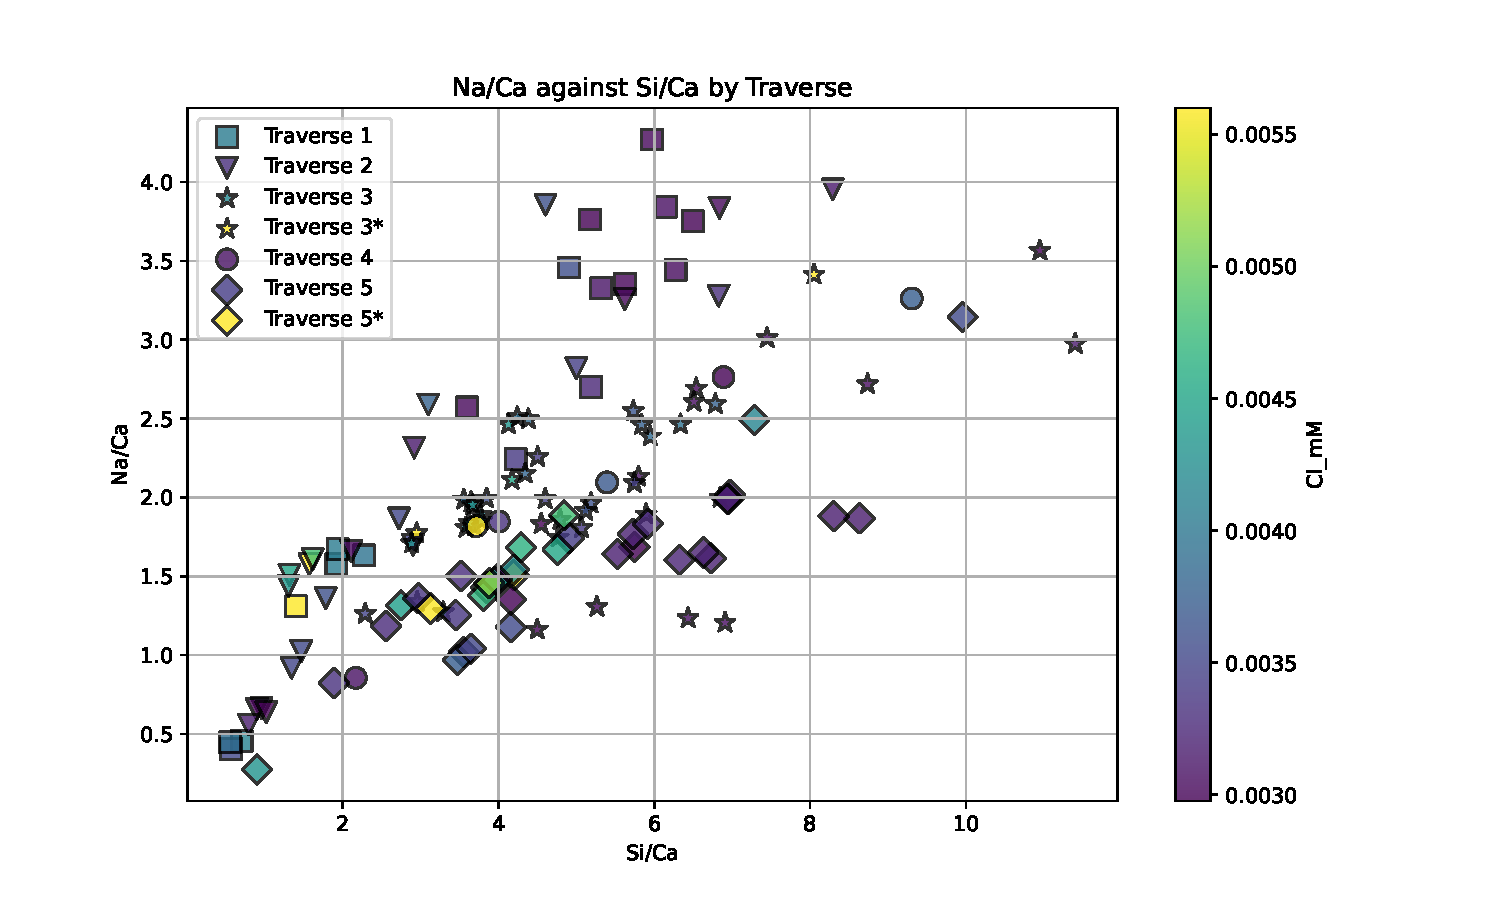
\includegraphics[width=\textwidth]{SiCaNaCa.pdf}
%     \caption{Si/Ca against Na/Ca. Clear differences between traverses.}
%     \label{fig:spatial_changes_spring3}
% \end{figure}


\begin{figure}[h]
    \centering
    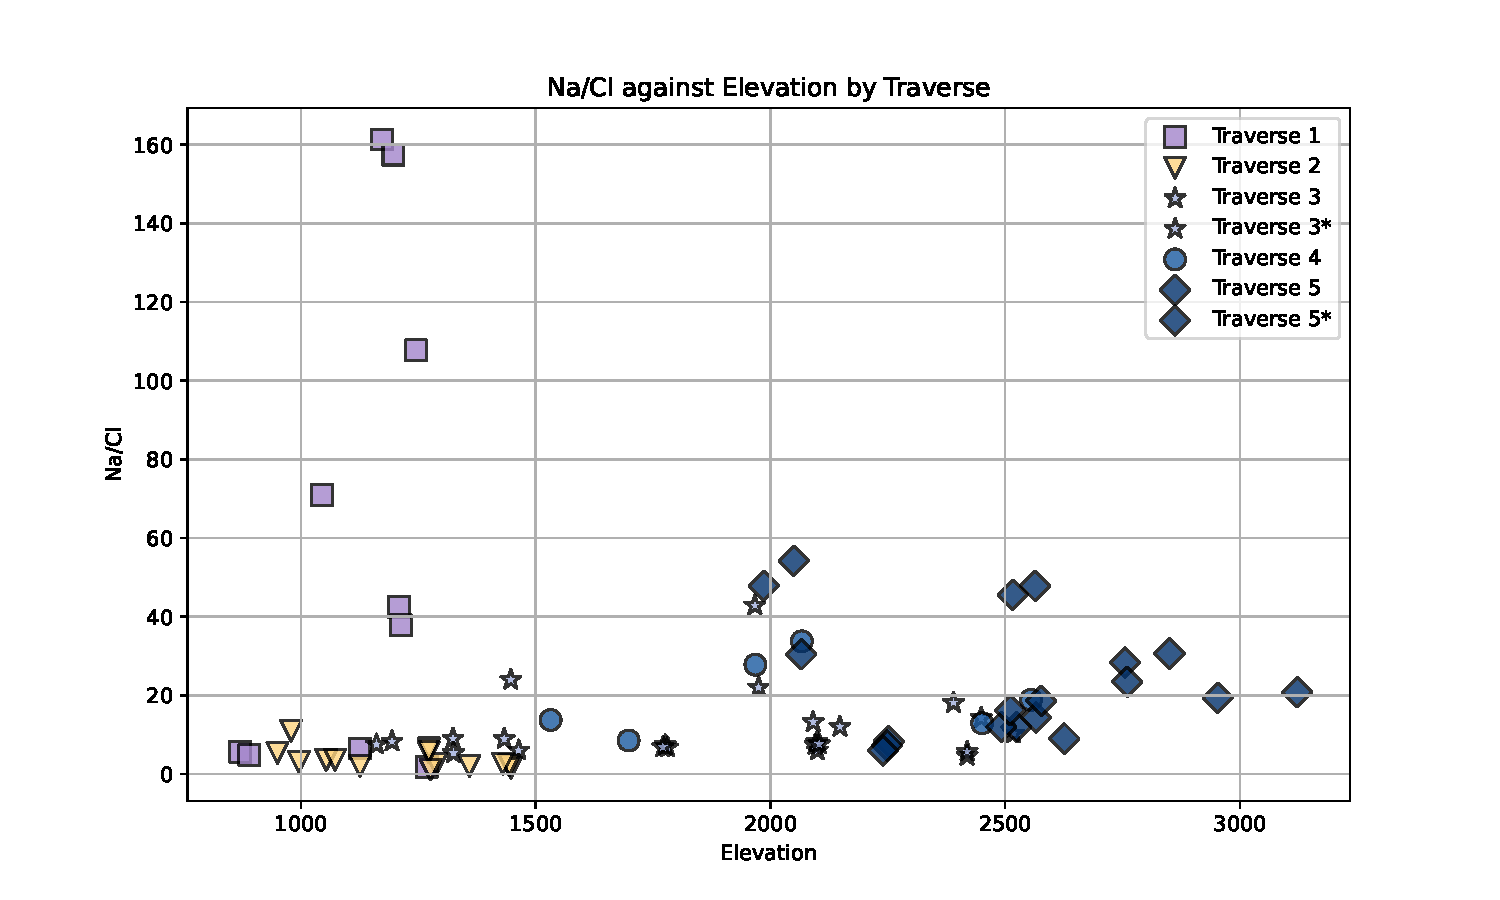
\includegraphics[width=\textwidth]{NaClEl.pdf}
    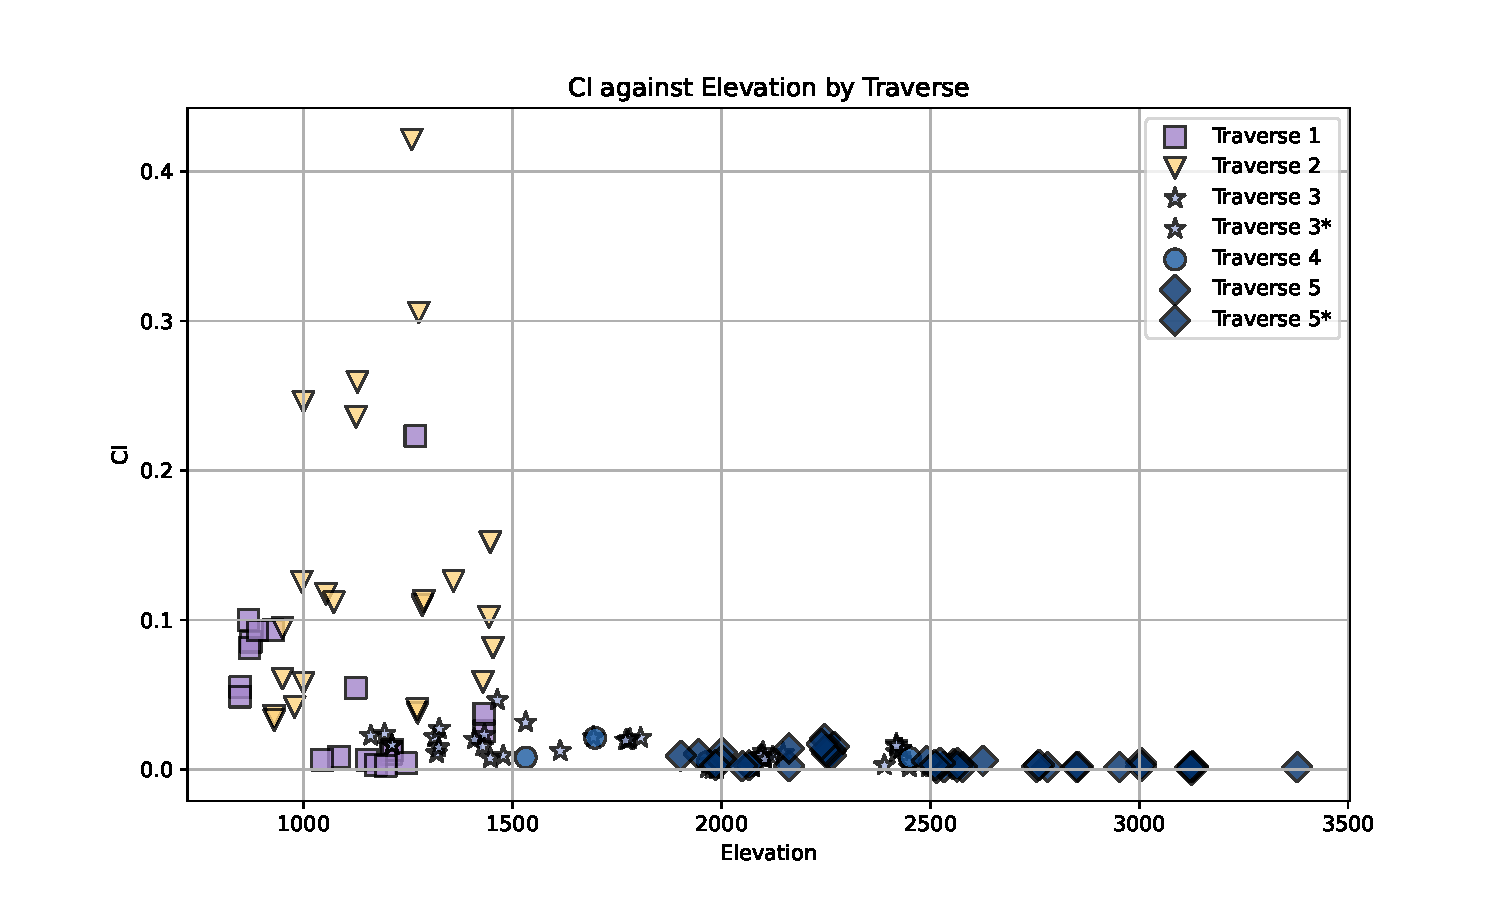
\includegraphics[width=\textwidth]{ClEl.pdf}
    \caption{NaCl against elevation coloured by traverse -  super low Cl; Cl against elevation coloured by traverse - Potential evaporite influence on traverse 2 water chemistry}
    \label{fig:spatial_changes_spring5}
\end{figure}

\FloatBarrier



\subsection{Sr isotope against 1/Sr data}
To eliminate evaporation, shows the differences between the springs.


\begin{itemize}
    \item Rain contribution suggests not much dust gets there at high elevations. Where is the cloud cover here?
    \item Sr against 1/Sr plot, suggesting springs are sampling different things with distance from the source. after Galy, France Lanord and Derry
\end{itemize}

Sr isotopes derived from the most recent rain analyses are of the order of 0.70904 to 0.70925 at the lowest. Seawater is of the order of 0.70917. Within error, therefore, the lowest rain values reflect seawater values, indicating little contamination from dust or particles. These are indeed found at the higher elevations \\


Also recreeate the plot from Galy, France Lanord and Derry 1998
\begin{figure}[h]
    \centering
    \begin{tabular}{cc}
        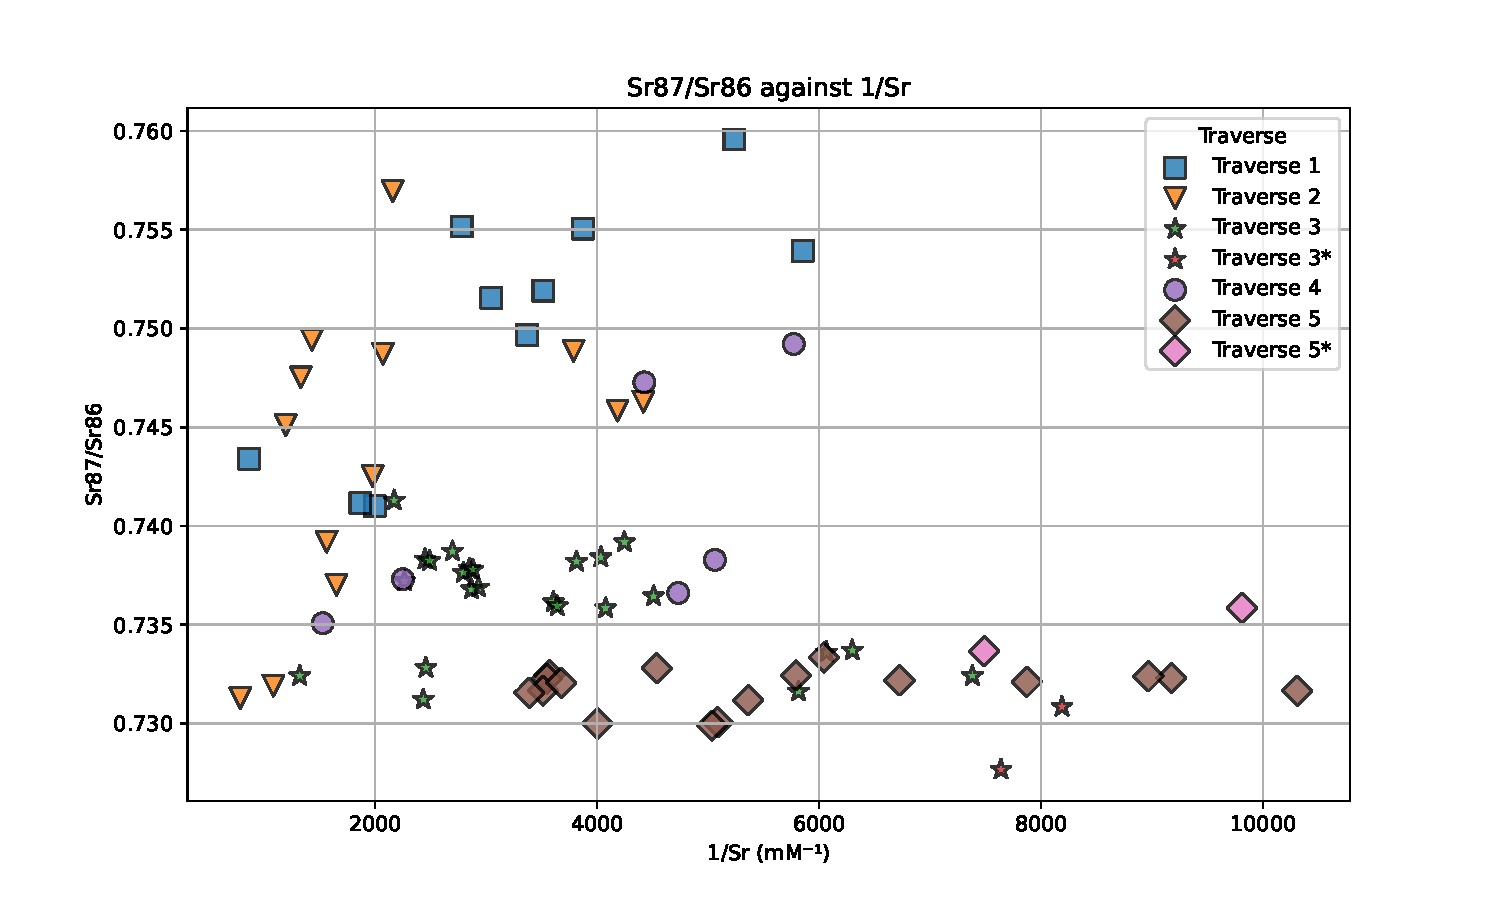
\includegraphics[width=0.5\textwidth]{Sr87_Sr86_1_Sr.pdf} & 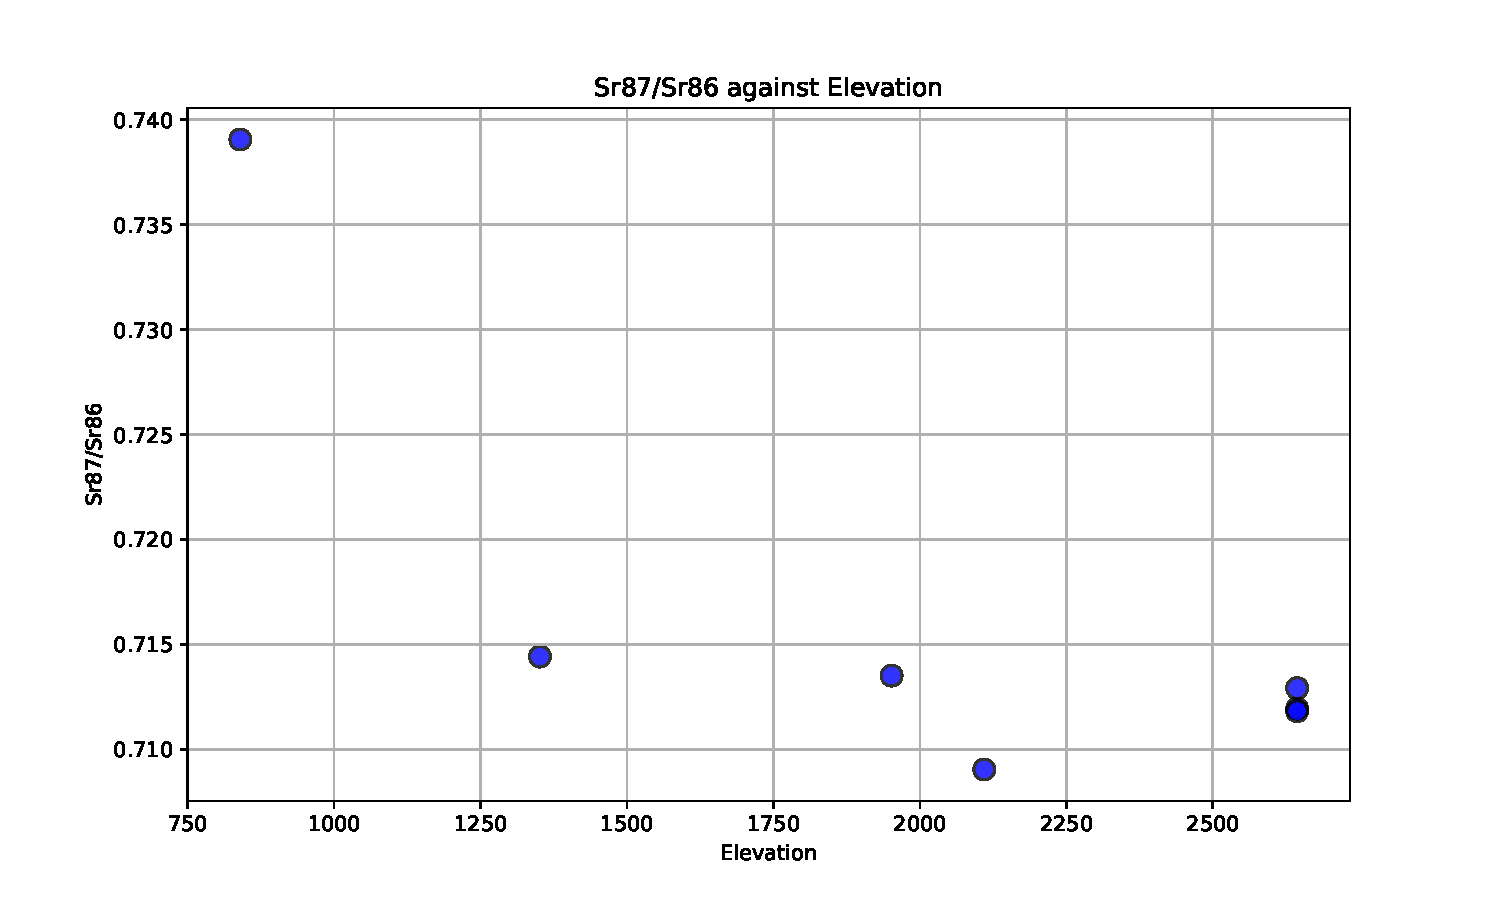
\includegraphics[width=0.5\textwidth]{Sr87_Sr86_Elevation.pdf} \\
        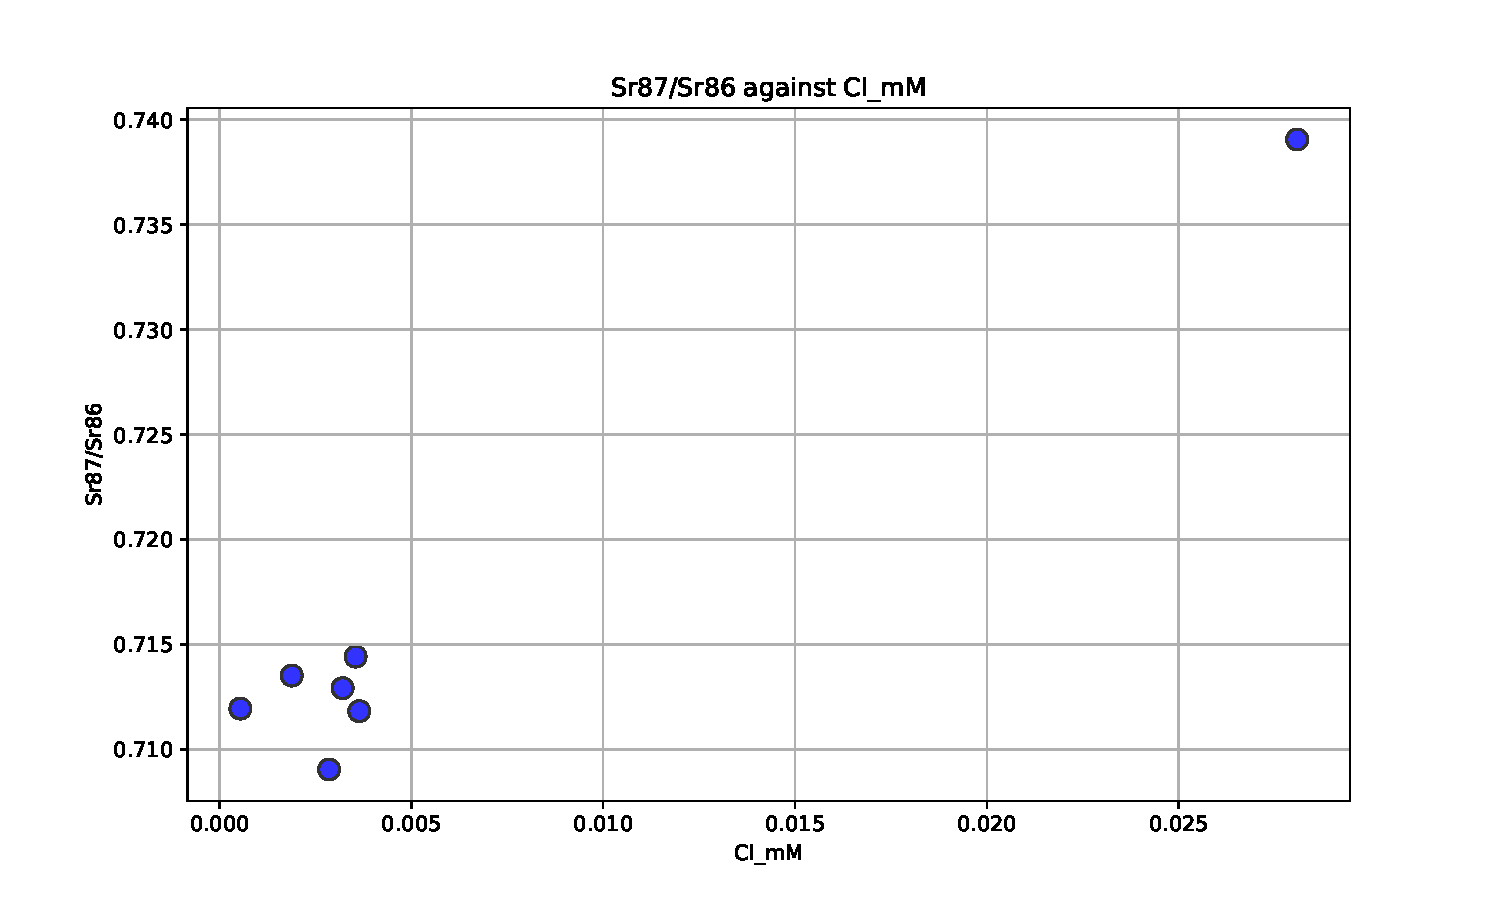
\includegraphics[width=0.5\textwidth]{Sr87_Sr86_Cl.pdf} & 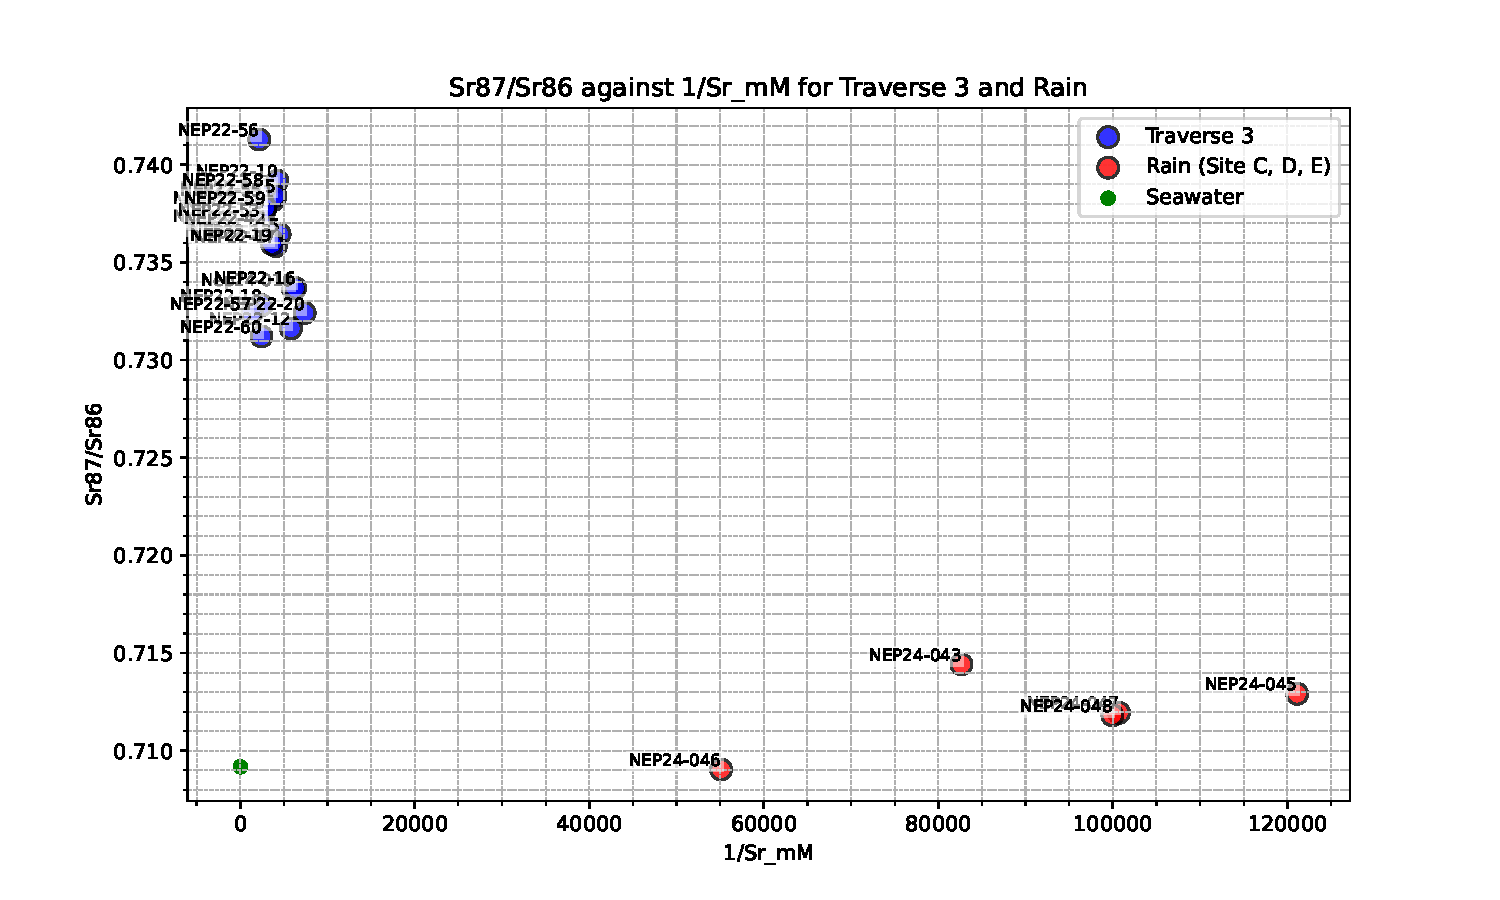
\includegraphics[width=0.5\textwidth]{Sr87_Sr86_1Sr_Rain.pdf} \\
    \end{tabular}
    \caption{Strontium isotope differences display difference in lithology tapped in. Cite Quade and Tipper papers; Rain analysed for Sr isotopes and Cl. Something about contamination lower down; How samples of Traverse 3 compare to the rain samples}
    \label{fig:discussion3}
\end{figure}

\FloatBarrier

% \begin{figure}[h]
%     \centering
%     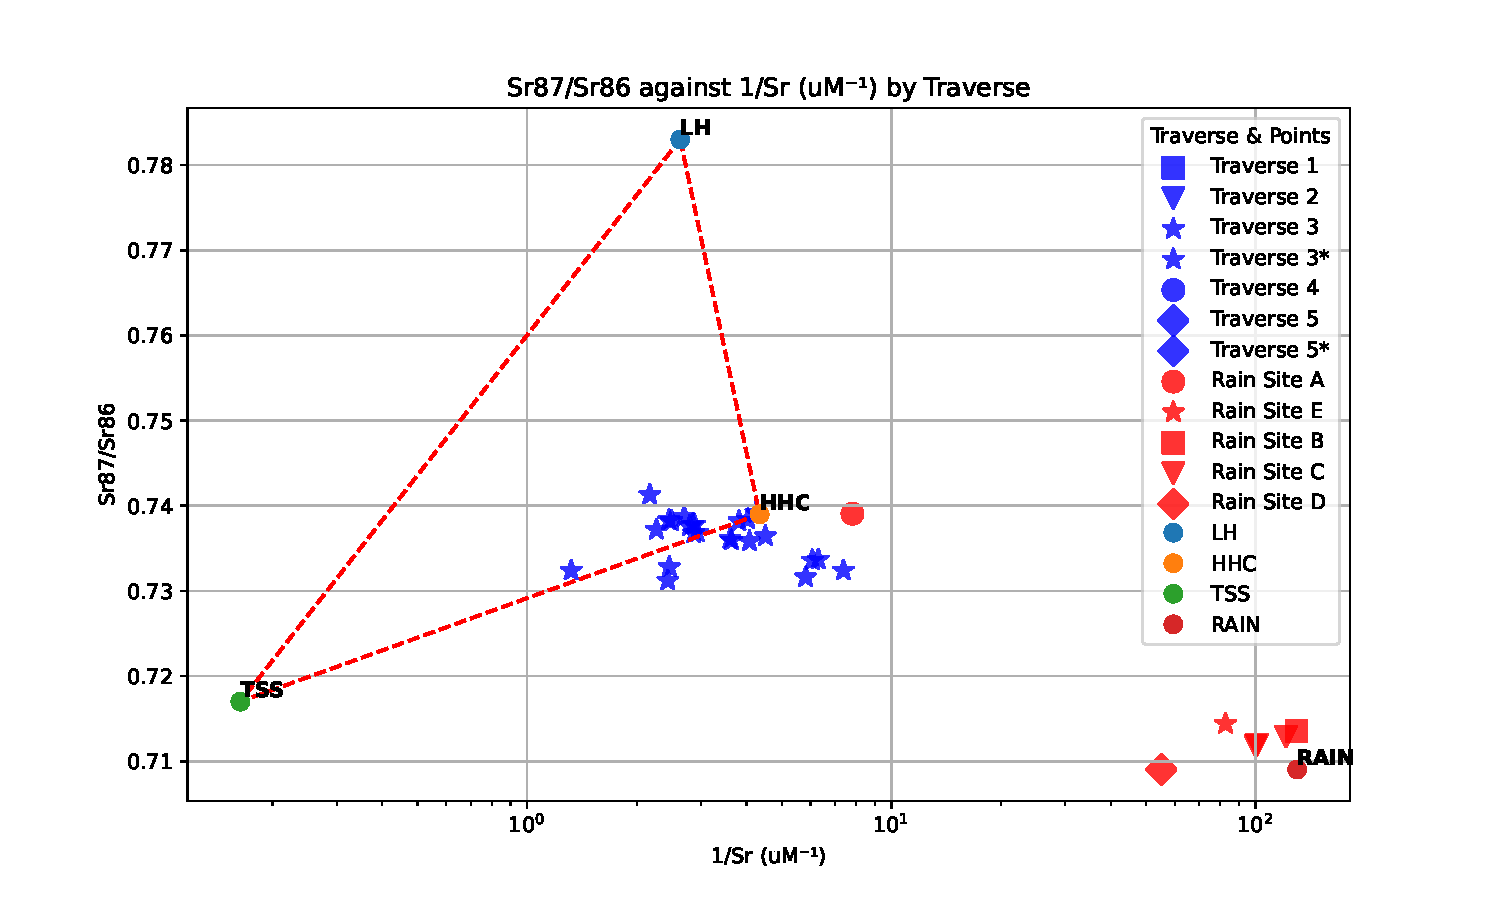
\includegraphics[width=\textwidth]{Sr87_Sr86_1Sr_Traverse_Triangle.pdf}
%     \caption{Recreating the Lanord plot etc. Need to choose better endmembers}
%     \label{fig:discussion4}
% \end{figure}

Also include 87Sr/86Sr weathering according to that mass balance thing... if that helps

\subsection{Traverse 3 is the best sampled and least influenced}
This will be modelled.

\begin{figure}[h]
    \centering
    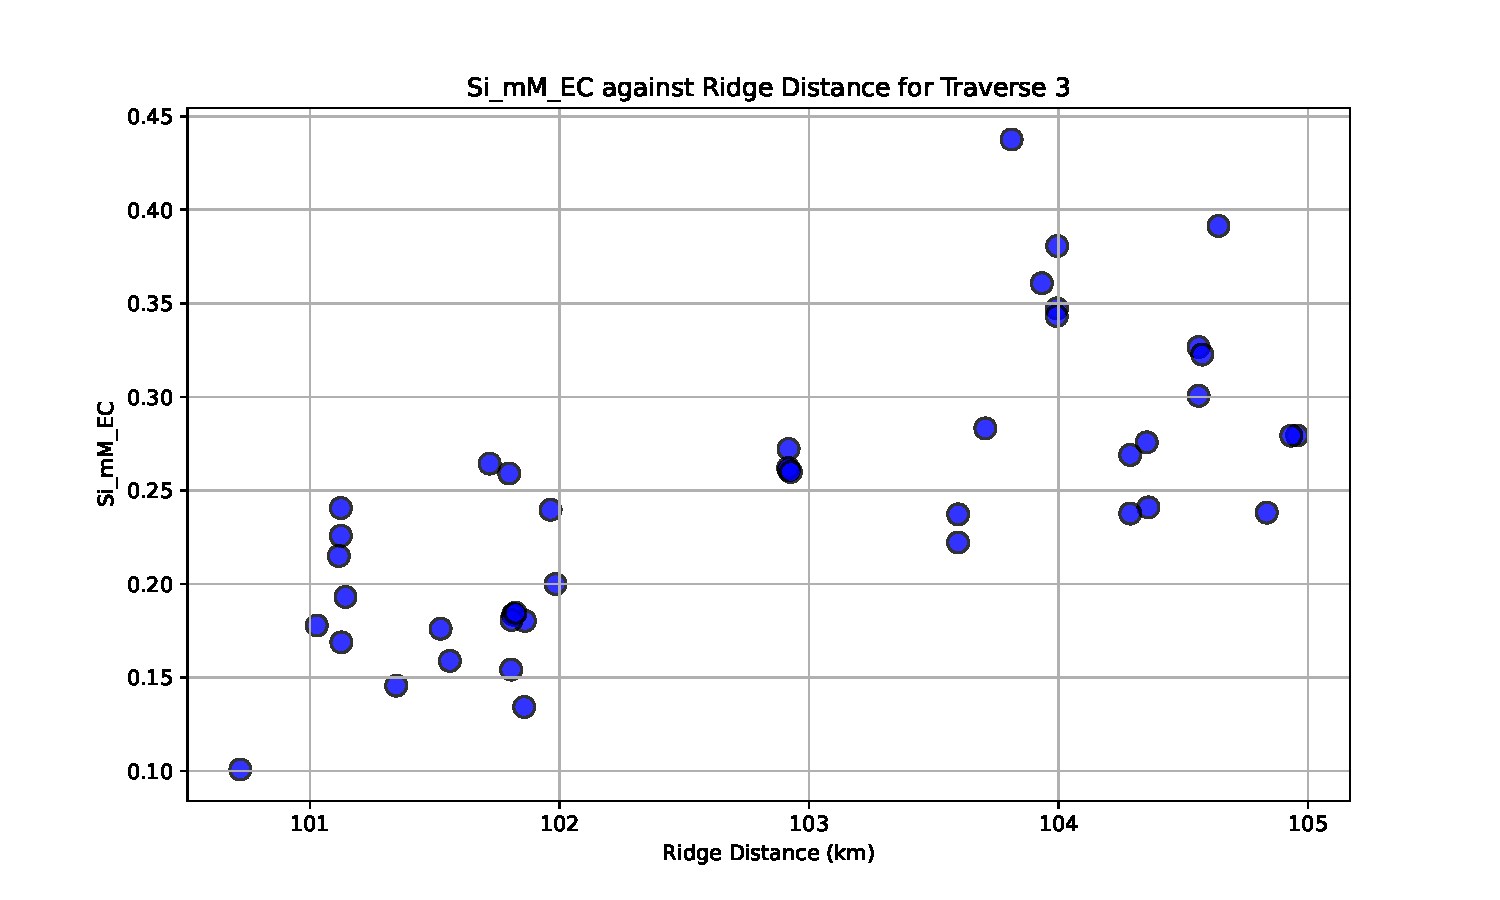
\includegraphics[width=\textwidth]{Si_mM_EC_Ridge_Distance.pdf}
    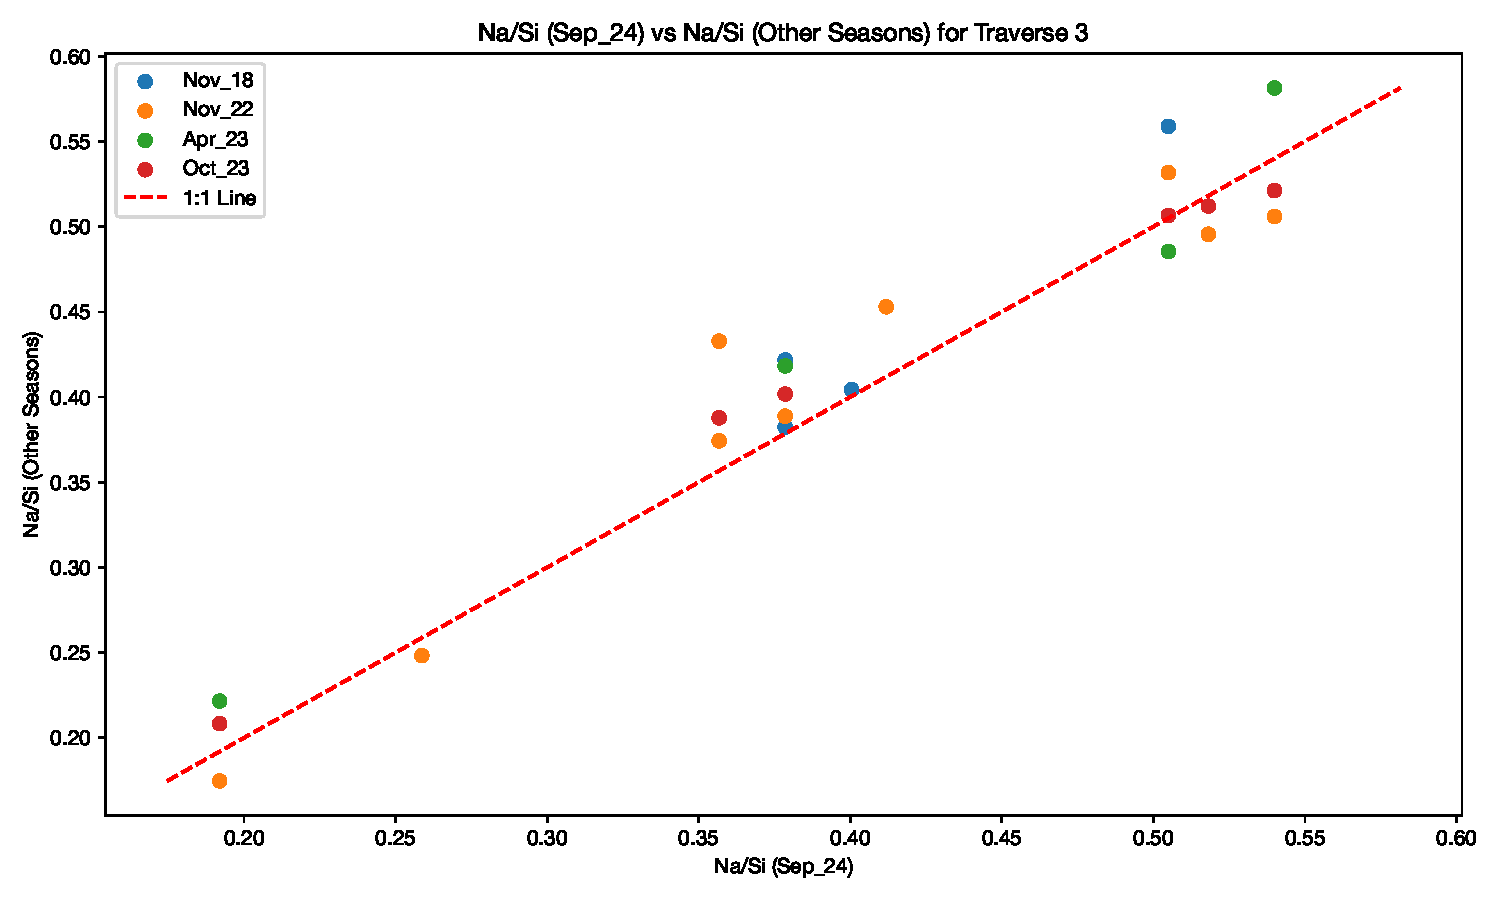
\includegraphics[width=\textwidth]{Na_Si_Trav3.pdf}
    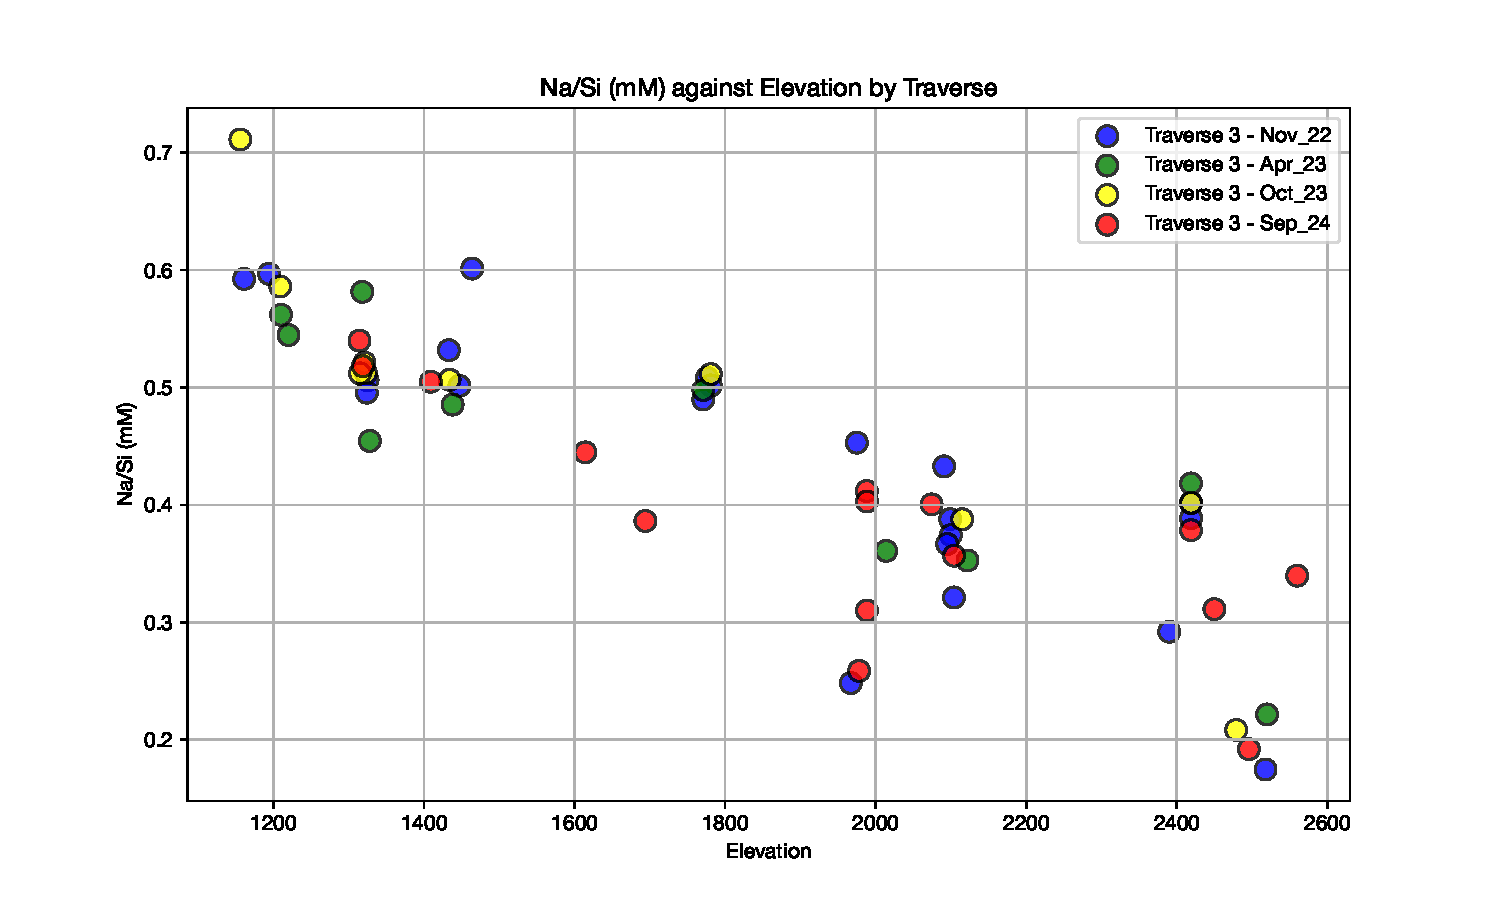
\includegraphics[width=\textwidth]{Na_Si_Elevation.pdf}
    \caption{How Si varies for Traverse 3, and showing the wide variety of samples; Na/Si for Traverse 3 is pretty neat; Na/Si for Traverse 3 is pretty neat. Consistently sampled flow paths}
    \label{fig:spatial_changes_spring8}
\end{figure}

\FloatBarrier


% \begin{figure}[h]
%     \centering
%     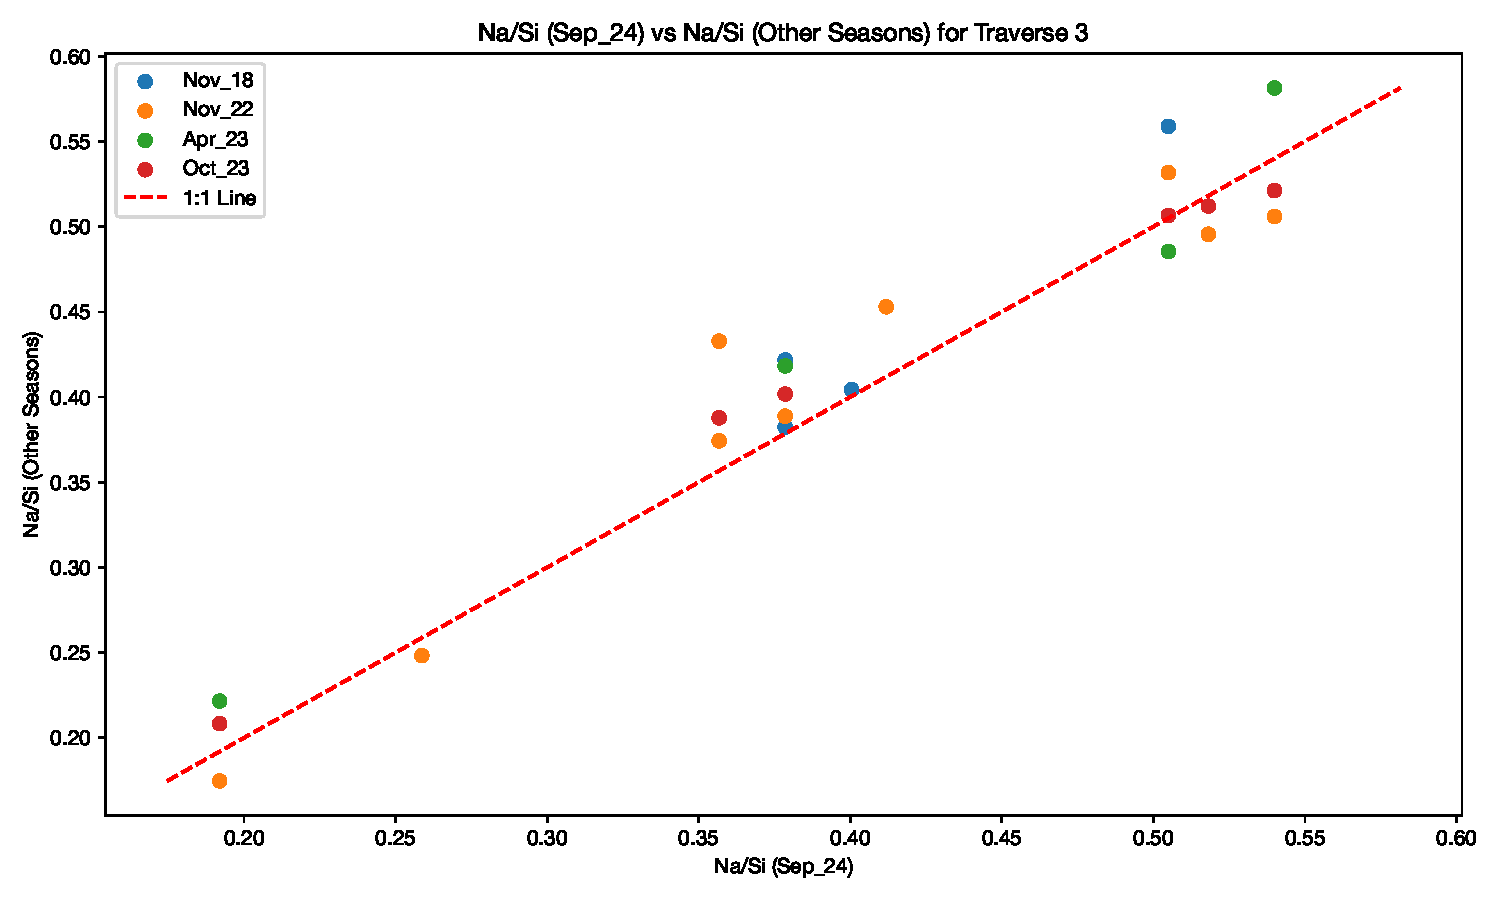
\includegraphics[width=\textwidth]{Na_Si_Trav3.pdf}
%     \caption{Na/Si for Traverse 3 is pretty neat}
%     \label{fig:spatial_changes_spring9}
% \end{figure}

% \FloatBarrier



